\chapter{Analisis dan Perancangan}

Pada bab ini diuraikan analisis yang telah dilakukan untuk mendapatkan rancangan solusi. Pada bagian analisis diuraikan analisis permasalahan, batasan masalah, dan analisis kebutuhan. Kemudian bab ini dilanjutkan dengan rancangan solusi berupa rancangan sistem dan rancangan \textit{rule} yang berdasarkan analisis yang telah dilakukan.

\section{Analisis Permasalahan}
Untuk mencapai tujuan pada pada subbab I.3, terdapat tiga komponen permasalahan: infeksi malware, deteksi malware dan penangkalan infeksi.

\subsection{Deteksi Infeksi Malware}

Dalam penelitian ini, sebuah host disebut terinfeksi oleh malware jika sebuah perilaku \textit{malicious} dari malware dilakukan oleh host tersebut. Host dapat berupa skala mesin komputer atau sebuah executable. Berbeda dengan \textit{compromised host} yang berarti ketika \textit{attacker} mendapatkan akses terhadap host. 

Analisis permasalahan pada bagian ini akan menjelaskan bagaimana tantangan yang dihadapi oleh pendekatan deteksi dalam mendeteksi malware. Pendekatan pada analisis ini akan menggunakan jenis-jenis pendekatan yang digunakan pada \cite{idika2007survey}. Jenis malware virus, worm dan bot akan menjadi fokus dari analisis karena perbedaan pendekatan yang dapat dilakukan untuk mendeteksi nya.

Menurut (\cite{6620049}), deteksi malware dikategorikan menjadi tiga, yakni: \textit{signature-based}, \textit{behavior-based}, dan \textit{heuristic-based}. \textit{Signature-based}, \textit{behavior-based}, dan \textit{Heuristic-based} pada (\cite{6620049}) dapat disamakan dengan \textit{static signature-based}, \textit{dynamic signature-based}, dan \textit{anomaly-based} berurutan pada (\cite{idika2007survey}). Dalam penelitian ini istilah yang digunakan mengacu pada (\cite{idika2007survey}).

Deteksi dengan menggunakan teknik \textit{anomaly-based detection} memiliki kelebihan dapat mendeteksi malware yang tidak dikenali. Namun deteksi dengan menggunakan teknik ini tidak dapat diaplikasikan secara praktis karena memiliki tingkat \textit{false-alarm} (\textit{false-positive}) yang tinggi. \textit{False-alarm} menjadi ancaman untuk \textit{availability} sistem jika \textit{action} dari \textit{rule} melakukan \textit{disable} terhadap sistem, ataupun koneksi.

Pada kasus malware dengan kelas virus, teknik-teknik seperti \textit{obfuscation}, enkripsi, \textit{oligomorphic}, \textit{polymorphic}, dan \textit{metamorphic} menjadikan deteksi dengan menggunakan static signature-based menjadi lebih sulit dilakukan.  Virus dengan teknik \textit{obfuscation} dapat ditemukan \textit{static signature}-nya dengan membersihkan \textit{garbage}. Sedangkan pada virus dengan teknik enkripsi umumnya melakukan pengubahan kunci enkripsinya sehingga bagian kode malicious tidak dapat dijadikan sebagai \textit{static signature}. Namun karena terdapat algoritma \textit{cipher} yang sama, maka hal tersebut dapat menjadi \textit{static signature}. Begitu pula pada teknik oligomorph dapat dideteksi dengan mendaftarkan seluruh algoritma \textit{cipher} yang digunakan malware sebagai \textit{static signature}. Sedangkan pada teknik \textit{polymorphic} dan \textit{metamorphic} deteksi dengan pendekatan deteksi statis sulit dilakukan.

Worm yang diklasifikasikan dengan karakteristik penyebaran mungkin memiliki teknik menyembunyikan diri dari deteksi dengan pendekatan \textit{static}. Worm dapat memiliki teknik-teknik yang dimiliki virus seperti dibahas sebelumnya. Sehingga worm dapat dikatakan sebagai salah satu subkelas dari virus yang memiliki kemampuan untuk berdiri sendiri dalam bentuk executable.

Deteksi worm dengan menggunakan \textit{dynamic signature-based} mungkin untuk dilakukan pada skala host atau pun \textit{network}. Pendekatan \textit{dynamic signature-based} dapat dilakukan generalisasi tidak hanya untuk mendeteksi malware dalam bentuk \textit{executable} namun dapat digunakan pada sekala host. Deteksi dengan pendekatan ini dapat digunakan untuk menentukan apakah sebuah host (mesin) telah terinfeksi, atau juga dapat digunakan dalam sekala sistem. 

Deteksi dengan \textit{dynamic signature-based} dapat digolongkan menjadi dua \textit{stateful} dan \textit{stateless detection}. Pada \textit{stateless detection}, sistem menentukan sebuah host atau executable \textit{malicious} hanya menggunakan informasi yang didapatkan pada saat itu. Deteksi \textit{stateless} ini dapat melakukan deteksi yang hemat sumber-daya. Namun, deteksi ini tidak dapat menemukan \textit{behavior} yang rumit dari sebuah malware. Sedangkan deteksi \textit{stateful dynamic signature-based}, menentukan sebuah host atau executable \textit{malicious} dengan menggunakan \textit{state} dan informasi yang didapatkan. Namun, deteksi jenis ini membutuhkan lebih banyak sumber-daya.

\subsubsection{Stateful dynamic signature-based detection}

\textit{Stateful dynamic signature-based detection} dapat direpresentasikan menggunakan state machine. State machine secara matematis dapat dimodelkan sebagai quintuple ($\Sigma$, $S$, $s_0$, $\delta$, $F$). $\Sigma$ sebagai himpunan alfabet input, $S$ sebagai himpunan state, $s_0$ sebagai state awal, $F$ sebagai himpunan state akhir, dan $\delta$ sebagai fungsi transisi yang memetakan $\delta : S \times \Sigma \rightarrow S$. 

Dalam deteksi penyebaran worm dalam jaringan menggunakan \textit{stateful dynamic signature-based detection} dapat menggunakan beberapa kategori state machine: \textit{connection-based state machine}, \textit{sender-based state machine}, \textit{target-based state machine}, \textit{pair-based state machine}.

Pada \textit{connection-based state machine}, State machine \textit{connection-based} memiliki ciri $s_0$ berupa state awal koneksi terbentuk, dan $\Sigma$ merupakan himpunan paket-paket \textit{signature} dalam koneksi tersebut. State machine dengan jenis ini dapat diterapkan untuk mendeteksi pada malware yang melakukan infeksi dalam satu buah koneksi.

Pada \textit{sender-based state machine}, $\Sigma$ merupakan himpunan paket \textit{signature} yang dikirim dari sebuah host. $s_0$ dapat berupa state ketika sebuah host mulai terlihat aktif dari sisi \textit{detector}, atau ketika detector baru diaktifkan seluruh host akan memiliki state ini. State machine ini dapat digunakan untuk mendeteksi host yang melakukan aktivitas \textit{malicious} sehingga bisa dijadikan alarm ketika host terinfeksi.

\textit{Target-based state machine} sedikit berbeda dengan \textit{sender-based state machine}, $\Sigma$ merupakan himpunan paket \textit{signature} yang diterima dari sebuah host. State machine ini dapat digunakan untuk mendeteksi ketika sebuah host diserang oleh beberapa host dengan pola tertentu. Namun state machine ini tidak memiliki state host yang melakukan serangan.

Pada \textit{$N$-tuple-based state machine}, $\Sigma$ merupakan himpunan yang paket signature pada komunikasi $N$-host. Jenis ini dapat mendeteksi ketika sebuah host diserang oleh beberapa host dengan pola tertentu, dan menyimpan state dari host mana serangan dilakukan. State machine ini lebih kompleks dari \textit{target-based state machine}.

\subsection{Penangkalan Infeksi Malware}

Proses penangkalan infeksi malware dapat dilakukan ketika deteksi telah dilakukan dan mendapatkan hasil positif. Untuk melakukan penangkalan infeksi malware, dapat dilakukan \textit{target-drop}, \textit{sender-drop}, atau \textit{connection-drop}. Teknik target-drop dan sender-drop dapat dilakukan ketika sebuah host di-indikasi diserang atau menyerang. Teknik ini dapat digunakan untuk mencegah infeksi meluas. Namun, teknik ini dapat mengganggu \textit{availability service} dan teknik ini jarang ditemui dalam penerapan. \textit{Connection-drop} merupakan teknik yang menghalangi koneksi terjadi ketika indikasi serangan ditemukan. Teknik ini merupakan teknik yang digunakan pada firewall.

\section{Analisis Perilaku Malware WannaCry}

Pada bagian ini, penulis melakukan analisis untuk mendapatkan \textit{signature} dari malware WannaCry, yang menjadi batasan masalah. Metodologi yang penulis lakukan sebagai berikut:

\begin{enumerate}
	\item {Melakukan studi literatur \textit{vulnerability} yang dieksploit oleh malware;}
	\item {Melakukan packet \textit{capture packet} yang dikirim oleh malware;}
	\item {Analisis hasil \textit{packet capture} terhadap studi literatur}
\end{enumerate}

\textit{Packet capture} pada lalu lintas paket malware WannaCry dilakukan dengan melakukan \textit{sniffing} dengan menggunakan 3 host dengan jaringan terisolasi seperti pada gambar \ref{fig:analisis_malware_net}.

\begin{figure}[H]
	\centering
	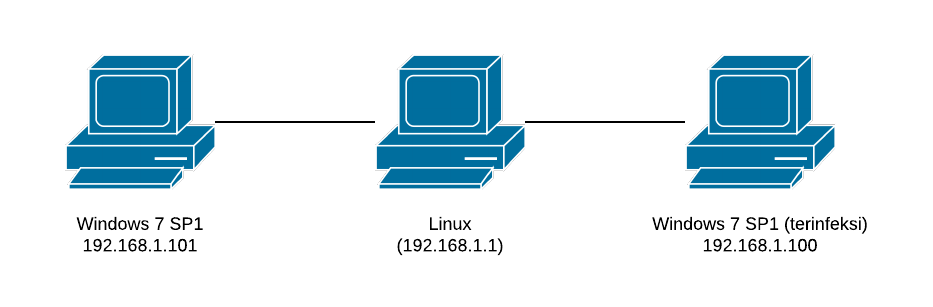
\includegraphics[width=400px]{resources/analisis_malware_net.png}
	\caption{Susunan jaringan untuk analisis malware WannaCry}
	\label{fig:analisis_malware_net}
\end{figure}

Host linux (192.168.1.1) merupakan host dengan dua \textit{interface} yang difungsikan sebagai \textit{bridge}. Sehingga host Windows 7 terinfeksi (192.168.1.100) dapat berkomunikasi dengan host Windows 7 (192.168.1.101) hanya melalui 192.168.1.1. Kemudian pada host linux dilakukan \textit{sniffing} dengan menggunakan tcpdump. dengan perintah sebagai berikut:

\begin{verbatim}
$ tcpdump -s0 -i br0 -vv -w output.wannacry-1.pcap
\end{verbatim}

\subsection{Hasil Studi Literatur}

Dari riset yang telah dilakukan oleh \cite{islam2018smb}, WannaCry melakukan exploit terhadap \textit{vulnerability} EternalBlue dan DoublePulsar yang ada pada implementasi SMB1. EternalBlue merupakan \textit{vulnerability} yang diakibatkan oleh 3 buah bug yang menurut (\cite{islam2018smb}) dan (\cite{grossman2017check}) yakni:
\begin{enumerate}
	\item Wrong casting bug
	\item Wrong parsing function bug
	\item Non-paged pool allocation bug
\end{enumerate}

Paket yang dikirimkan malware untuk mengeksploitasi vulnerability (\cite{islam2018smb}) yakni dengan mengirimkan \verb|SMB_COM_NT_TRANSACT|  diikuti dengan \verb|SMB_COM_TRANSACTION2_SECONDARY|.

\subsection{Analisis Hasil Packet Capture}

Berdasarkan pengelompokan malware menjadi worm, virus, dan \textit{trojan horse}; WannaCry digolongkan sebagai worm. Sesuai dengan karakteristik yang disebutkan dalam dasar teori, WannaCry memiliki kemampuan menginfeksi melalui jaringan.

WannaCry memiliki dua buah bagian utama: ransomware, dan worm penginfeksi, yang melakukan penyebaran melalui protokol SMB. Jika sebuah host hanya menjalankan bagian ransomware saja, maka tidak akan ada penyebaran yang dilakukan, seperti ditunjukan pada Gambar \ref{fig:no_infect_action}. Sedangkan jika host menjalankan bagian dropper, dropper tersebut akan menjalankan worm penginfeksi dan sekaligus menjalankan ransomware. Pada Gambar \ref{fig:infect_action} terlihat host 192.168.1.100  mencoba melakukan koneksi ke port \verb|445/tcp| setiap host yang berada pada subnet yang sama.

\begin{figure}[H]
	\centering
	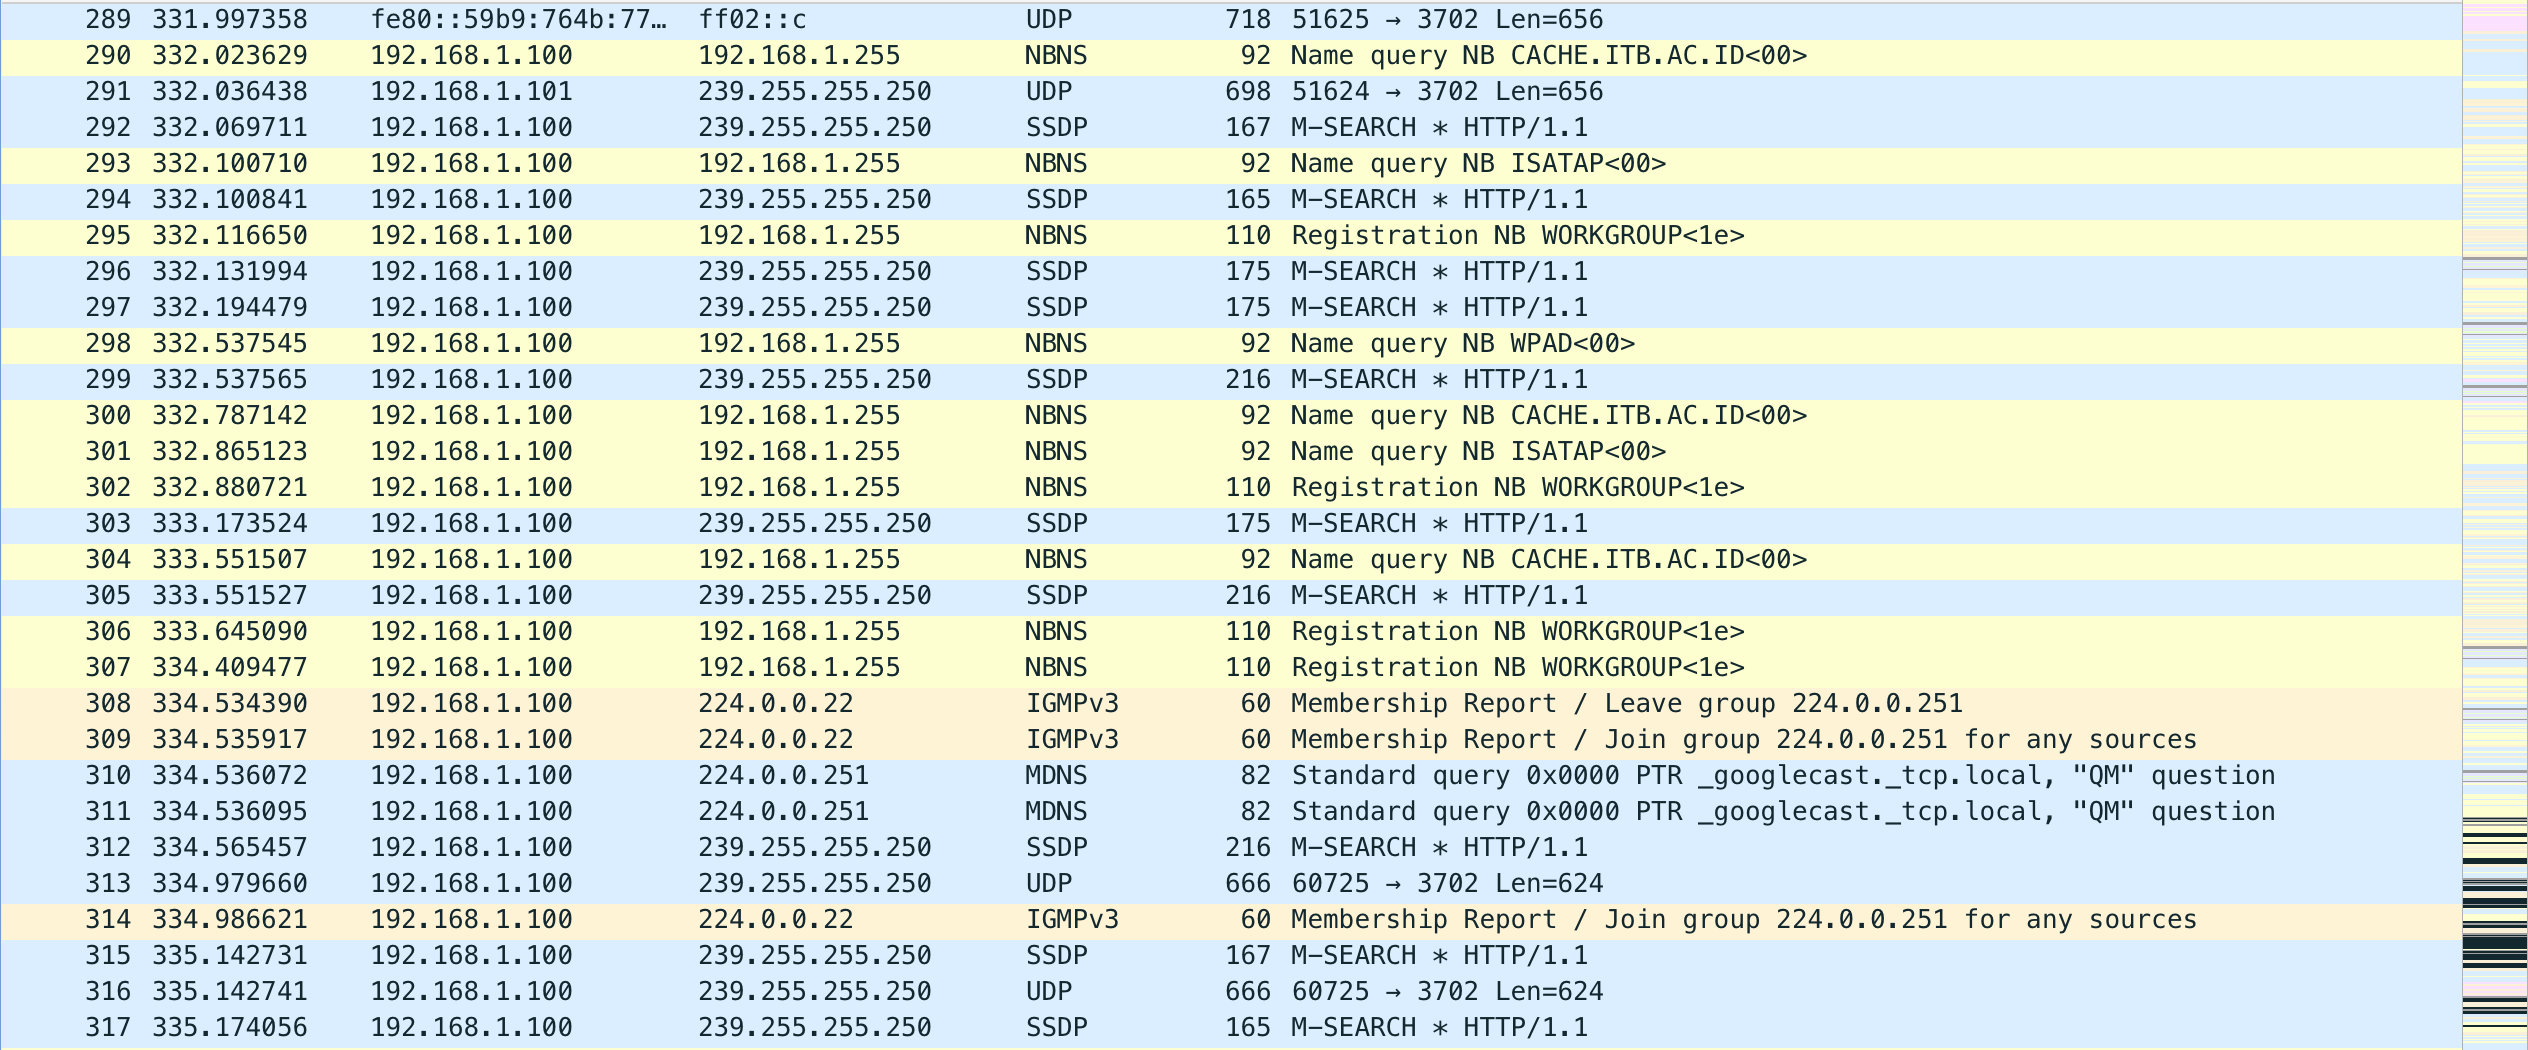
\includegraphics[width=\textwidth]{resources/no_infect_action.png}
	\caption{Paket pada host terinfeksi ransomware tanpa worm penginfeksi}
	\label{fig:no_infect_action}
\end{figure}

\begin{figure}[H]
	\centering
	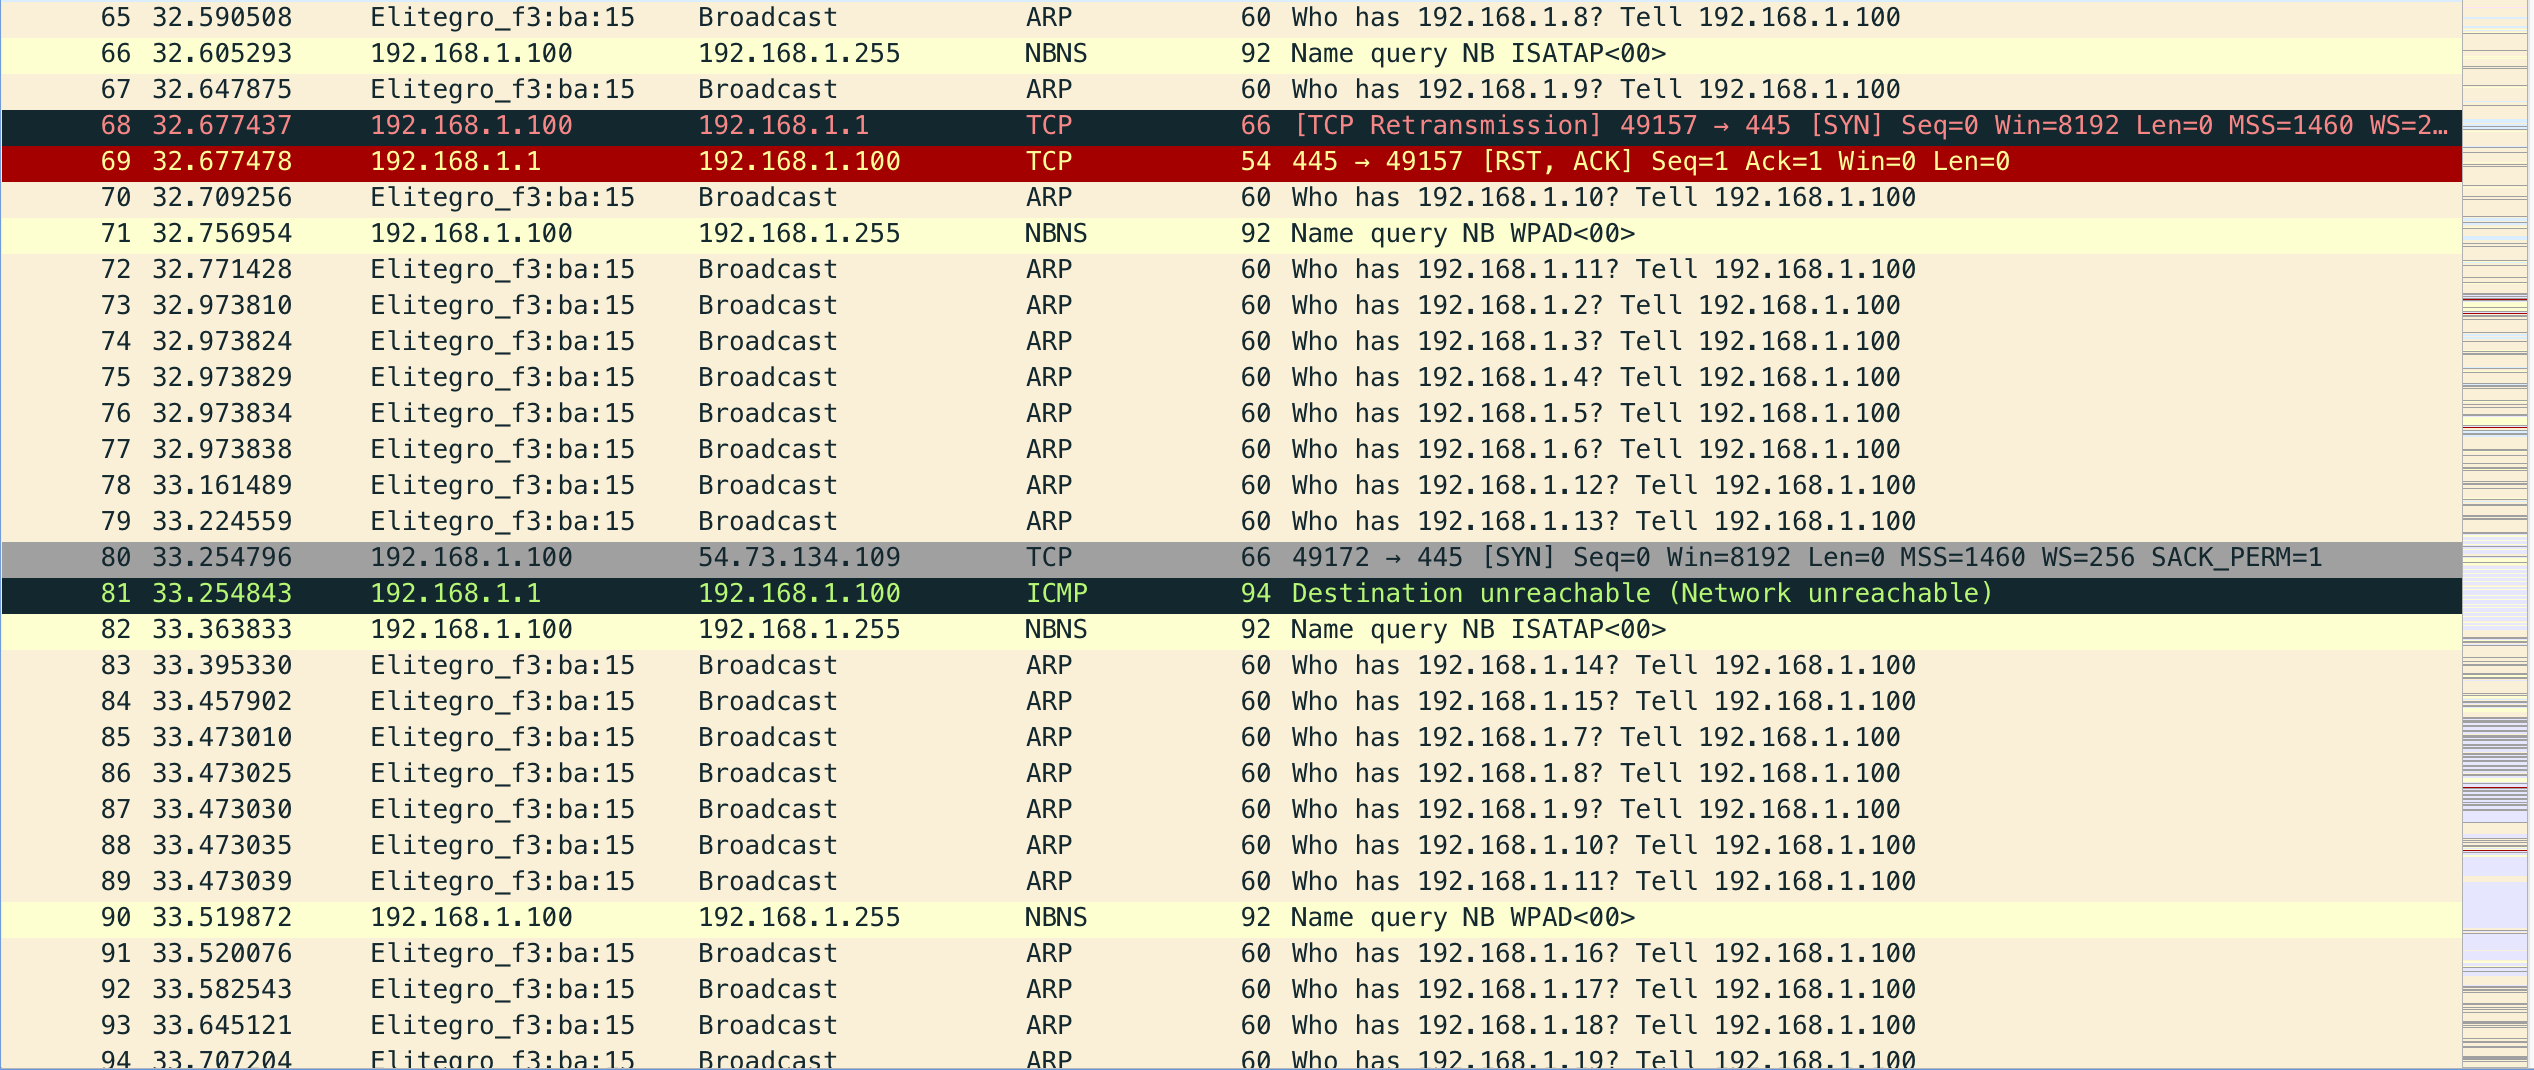
\includegraphics[width=\textwidth]{resources/infect_action.png}
	\caption{Paket pada host terinfeksi ransomware dengan dropper}
	\label{fig:infect_action}
\end{figure}

Ransomware merupakan kategori malicious software yang ketika dijalankan akan menonaktifkan fungsi tertentu dari komputer dengan sebuah cara. Kemudian ransomware akan menampilkan pesan untuk meminta pembayaran untuk mengembalikan fungsi yang dinonatifkan. Sehingga malware seakan-akan melakukan penyanderaan terhadap komputer. (\cite{o2012ransomware}).

Pada paket yang dikirimkan host 192.168.1.100 terlihat malware berusaha mengeksploitasi \textit{vulnerability} seperti yang disebutkan (\cite{islam2018smb}), yakni dengan mengirimkan \verb|SMB_COM_NT_TRANSACT| terlihat pada Gambar \ref{fig:trans_nop}, diikuti dengan \verb|SMB_COM_TRANSACTION2_SECONDARY| seperti pada Gambar \ref{fig:trans2_secondary}.

\begin{figure}[H]
	\centering
	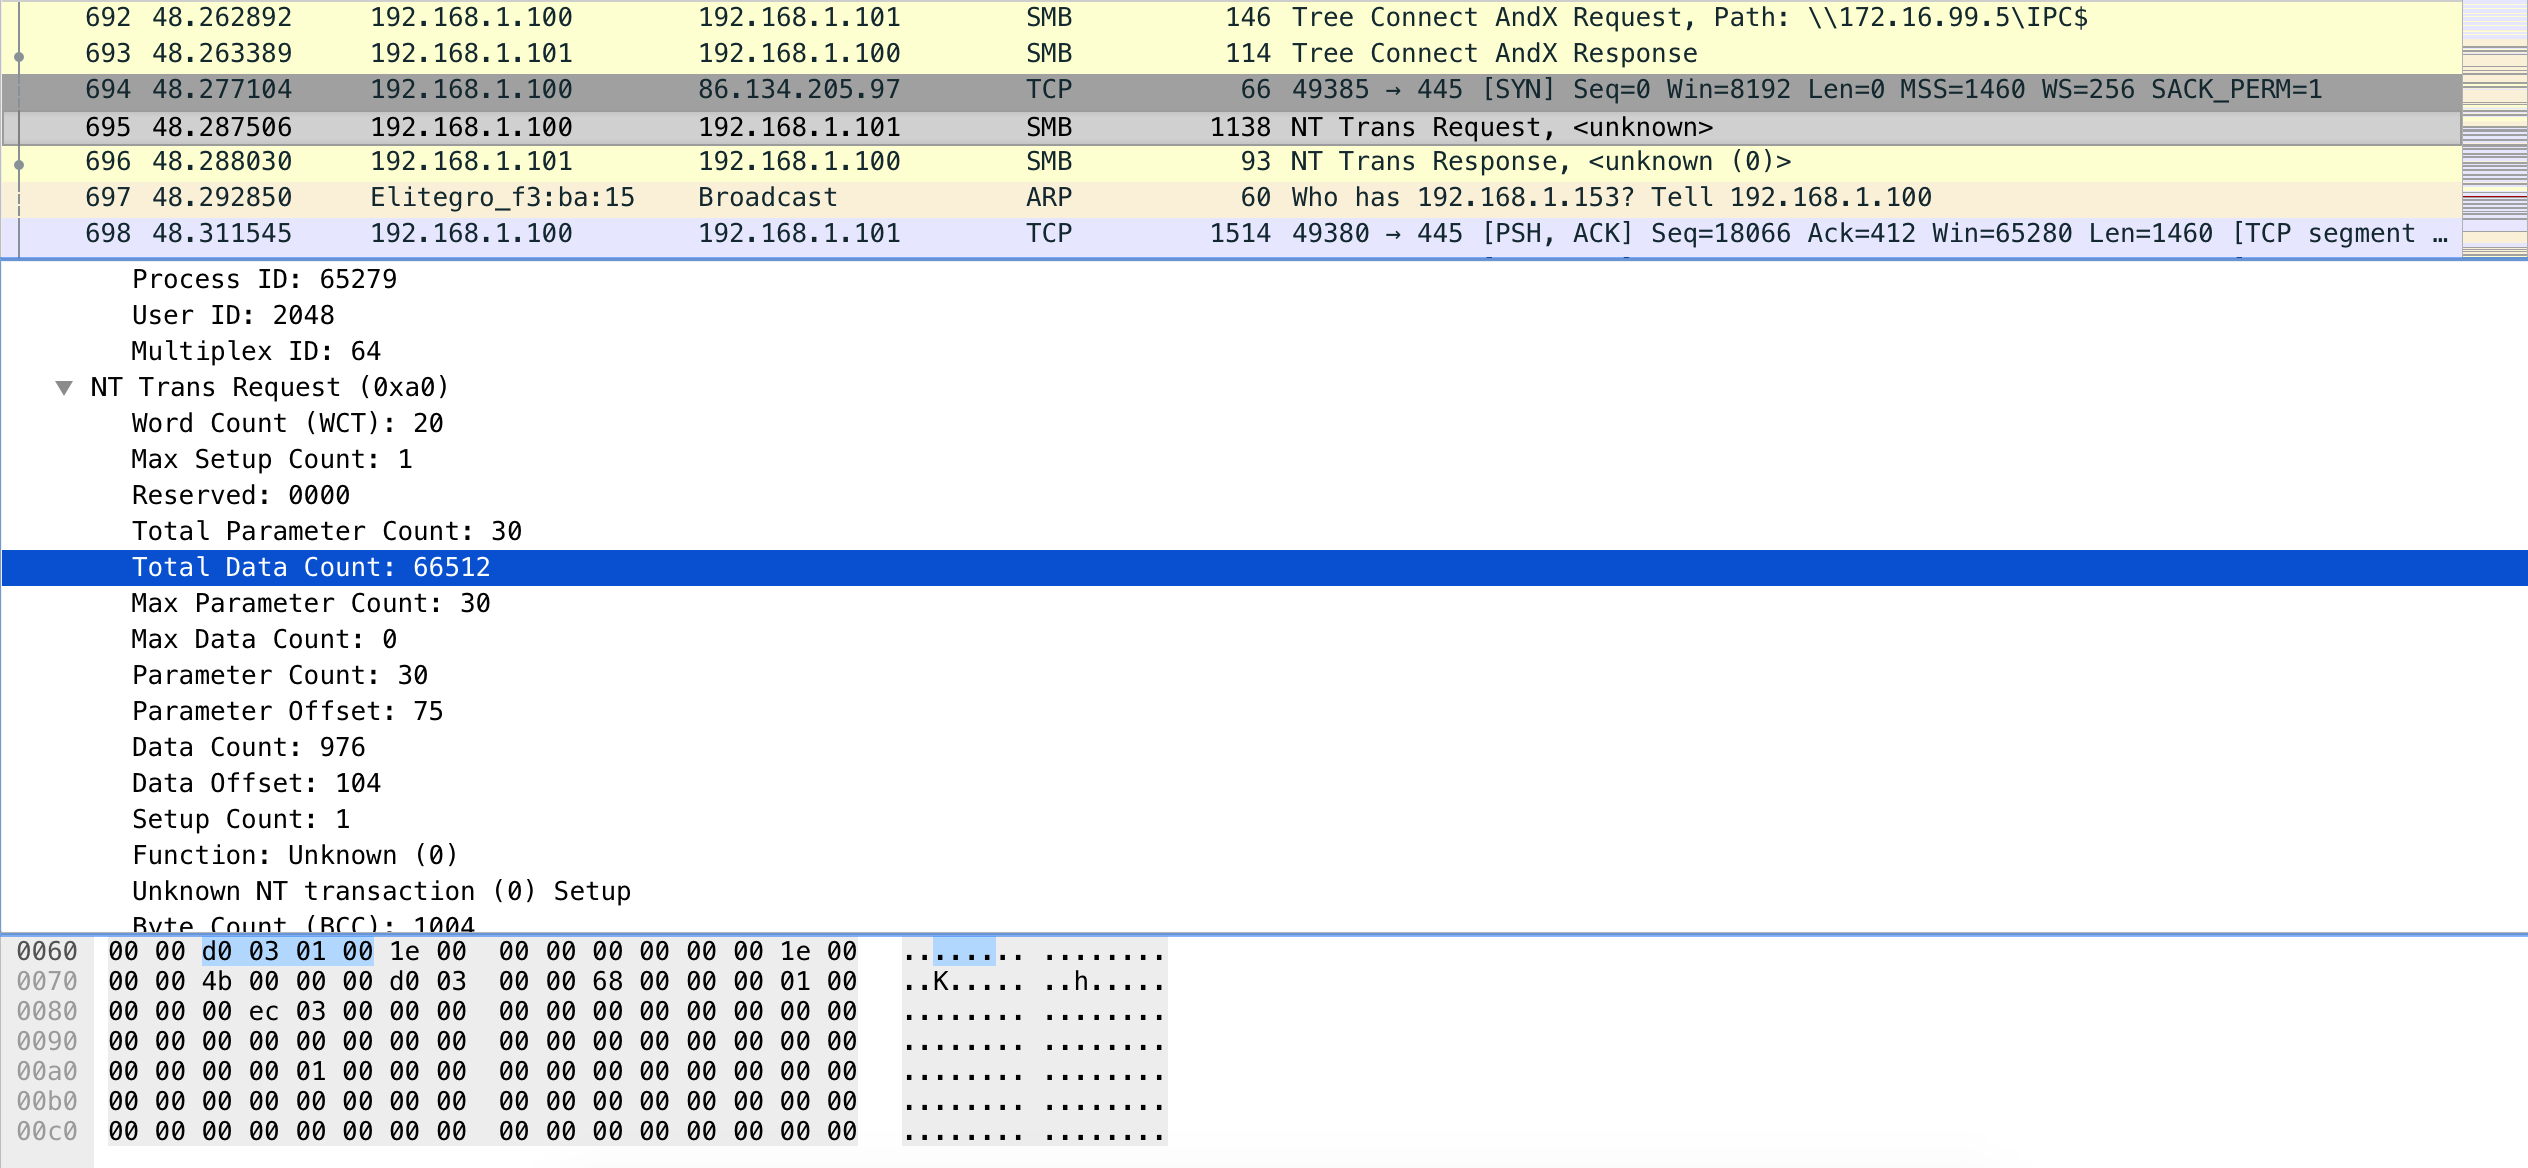
\includegraphics[width=\textwidth]{resources/trans_nop.png}
	\caption{Paket SMB\_COM\_NT\_TRANSACT dari host terinfeksi}
	\label{fig:trans_nop}
\end{figure}
\begin{figure}[H]
	\centering
	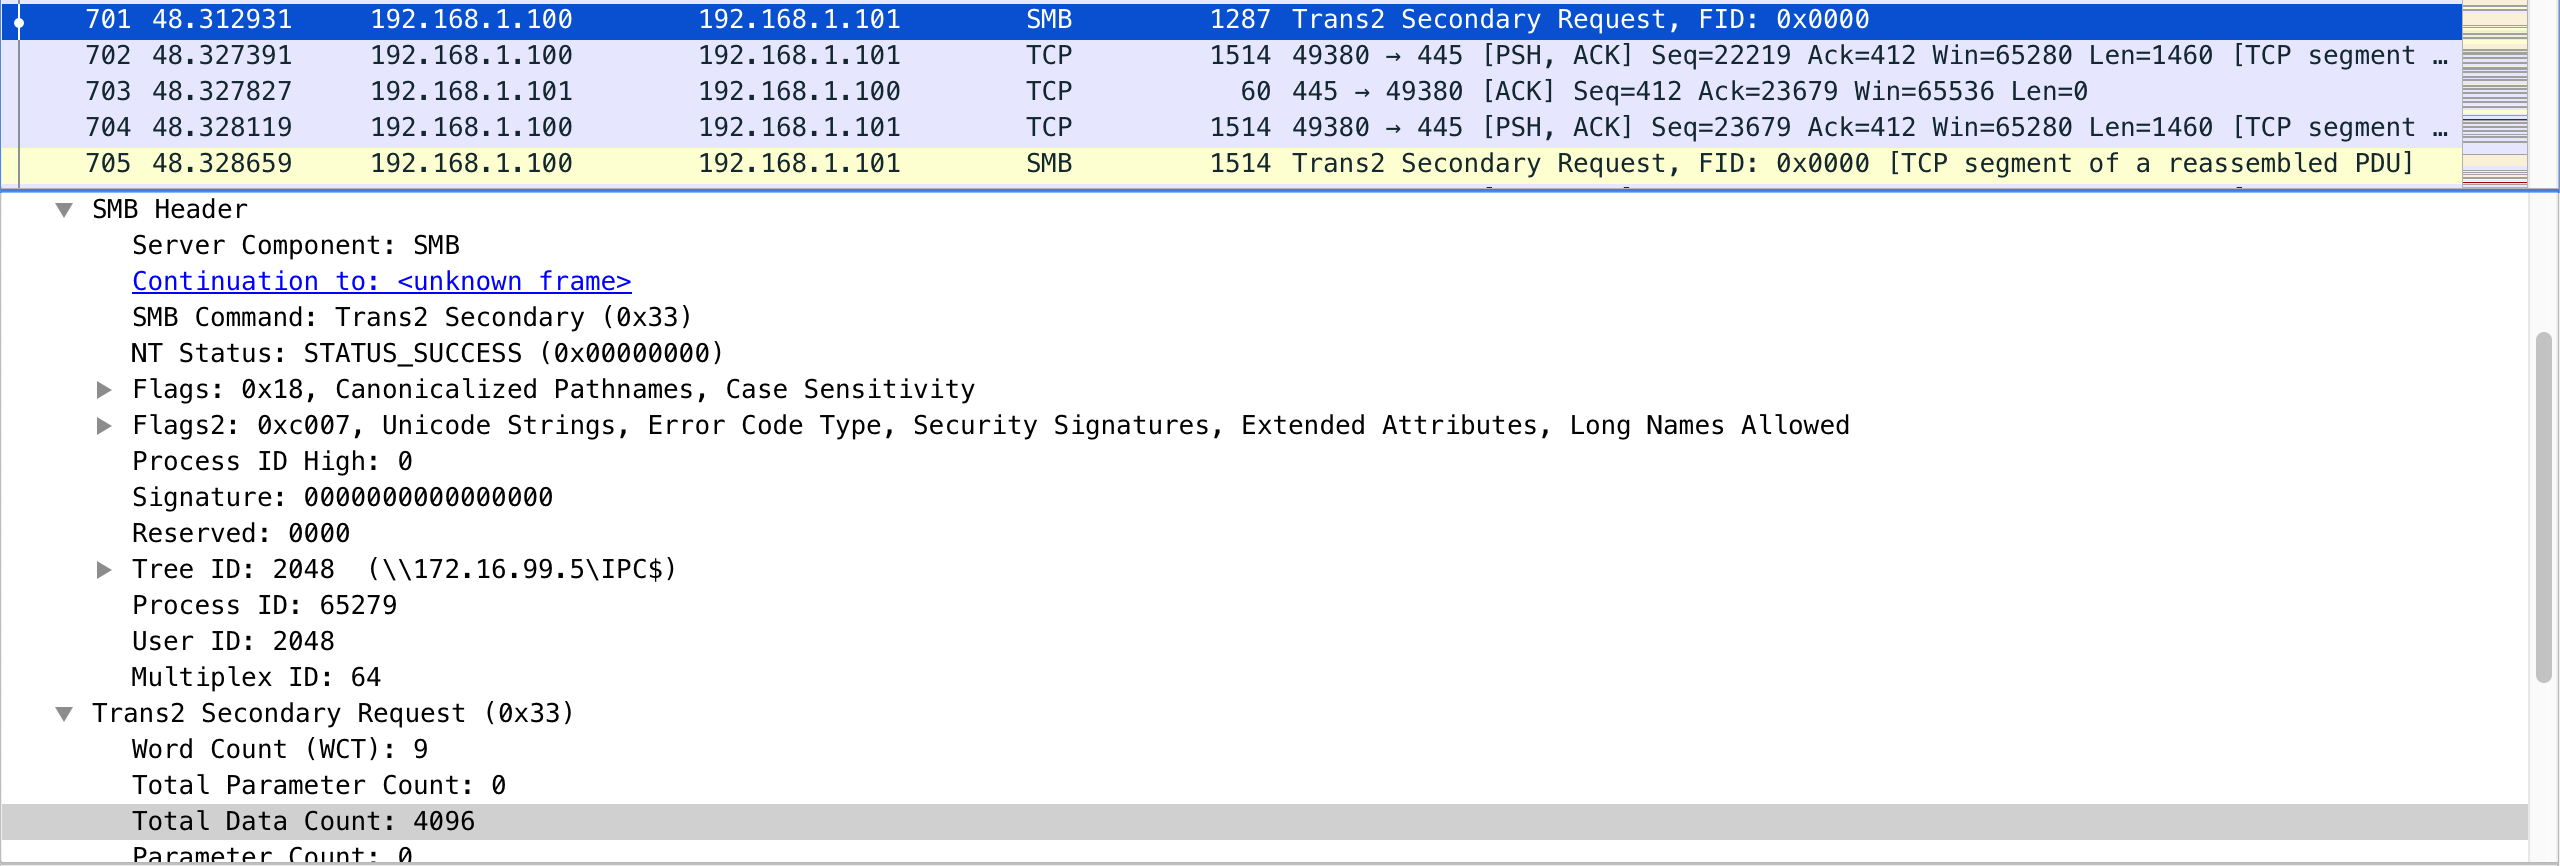
\includegraphics[width=\textwidth]{resources/trans2_secondary.png}
	\caption{Paket SMB\_COM\_TRANSACTION2\_SECONDARY dari host terinfeksi}
	\label{fig:trans2_secondary}
\end{figure}

Ketika \textit{payload} sebuah perintah tidak cukup untuk dimasukkan ke dalam satu paket \verb|SMB_COM_NT_TRANSACT|, seharusnya kelebihan ini dimasukkan ke dalam perintah \verb|SMB_COM_NT_TRANSACT_SECONDARY|. Tetapi WannaCry dengan sengaja menggunakan \verb|SMB_COM_TRANSACTION2_SECONDARY| sehingga menimbulkan \textit{wrong casting bug}. Kedua paket ini dapat dijadikan \textit{signature} untuk deteksi ketika ada malware yang ingin melakukan eksploit terhadap \textit{vulnerability} ini. Perlu sebuah kakas yang dapat mendeteksi jenis perintah yang digunakan oleh paket SMB.


\section{Analisis Kebutuhan}

Hasil analisis malware pada subbab sebelumnya untuk mencapai tujuan pada BAB I, diperlukan kakas yang dapat melakukan:

\subsection{Mekanisme Penangkalan Paket Malicious}

Ketika paket \textit{malicious} dapat dideteksi, harus ada suatu mekanisme yang dapat menangkal paket tersebut sehingga tidak sampai ke host yang dituju. Pada konteks ini, firewall seharusnya dapat melakukan penangkalan agar paket \textit{malicious} dapat dihentikan.

Kakas yang umum digunakan untuk melakukan penangkalan paket dalam bentuk firewall pada sistem operasi linux adalah iptables. Iptables seperti dijelaskan pada subbab II.7 memiliki struktur umum yang dapat digunakan untuk berbagai keperluan. Penangkalan pada iptables dapat dilakukan dengan membuat aturan yang memiliki \textit{action} DROP atau REJECT.

\subsection{Deteksi Protokol Layer Aplikasi}

Penangkalan terhadap aktivitas \textit{malicious} terhadap host lain dapat dilakukan dengan mendeteksi \textit{signature} yang terdapat pada paket yang dikirimkan. Untuk melakukannya, signature akan spesifik terhadap protokol layer aplikasi tertentu. Sehingga firewall harus dapat membedakan protokol yang digunakan pada layer aplikasi.

Deteksi jenis protokol layer aplikasi dapat dilakukan dengan menggunakan DPI seperti telah dibahas pada BAB II. Salah satu kakas yang umum digunakan adalah nDPI.

nDPI merupakan pengembangan OpenDPI (\cite{deri2014ndpi}). Jika dibandingkan dengan kakas lain, nDPI memiliki akurasi yang lebih tinggi seperti PACE, UPC MLA, dan Libprotoident (\cite{bujlow2013comparison}).

\subsection{State Machine}

Dari analisis malware yang telah dilakukan, untuk melakukan deteksi sebuah aktivitas \textit{malicious} dalam beberapa kasus tidak dapat ditentukan dari satu paket saja. Dalam kasus WannaCry dalam melakukan eksploitasi \textit{vulnerability} EternalBlue setidaknya perlu mendeteksi dua paket yakni \verb|SMB_COM_NT_TRANSACT| yang kemudian diikuti paket \verb|SMB_COM_TRANSACTION2_SECONDARY|.

Dengan menggunakan konsep state machine dan firewall yang melakukan pengecekan pada setiap paket, setiap paket dapat dikongruensikan sebagai alfabet pada state machine. Kemudian, bahasa yang diterima state machine merupakan semua aktivitas \textit{malicious} yang sesuai dengan signature.

\subsection{Deteksi Signature yang Paham terhadap Struktur Data}

Setelah diketahui jenis protokol yang digunakan, untuk dapat menangkal paket \textit{malicious} seperti yang digunakan WannaCry untuk melakukan penyebaran, diperlukan sebuah kakas yang dapat mendeteksi paket yang dikirimkan sesuai dengan struktur data paket tersebut. Dengan melakukan pendeteksian yang memahami struktur data paket diharapkan dapat memperkecil kesalahan deteksi.

Namun, kakas deteksi seperti \verb|match string| hanya melakukan pencocokan pada \textit{payload} dan tidak memiliki fitur untuk melakukan pencocokan pada bagian tertentu dari struktur data paket. Sehingga tidak dapat mendeteksi bagian seperti byte ke-n dari sebuah paket. Padahal hal ini diperlukan untuk melakukan pencocokan misalkan pada jenis perintah yang digunakan pada protokol SMB.

Berikut tabel \ref{table:software_requirement} yang merangkum kebutuhan perangkat lunak yang muncul untuk mencapai tujuan pada BAB I. Sebuah sistem penangkal malware memerlukan sebuah sistem penangkalan paket sehingga dapat melakukan penangkalan ketika dideteksi terjadi serangan. Selain itu sistem penangkal malware ini juga harus memiliki state machine untuk dapat melakukan pengecekan secara \textit{stateful}. Sebuah sistem penangkal malware ini juga harus memiliki deteksi protokol dan \textit{signature} pada level aplikasi sehingga dapat mendeteksi perilaku malware tidak hanya pada layer \textit{transport}. Kemudian sistem penangkal malware juga harus memiliki basis data untuk menyimpan \textit{signature}, sehingga perlu fungsionalitas menambahkan \textit{rule}.

\begin{table}[H]
	\caption{Tabel kebutuhan perangkat lunak}
	\label{table:software_requirement}
	\begin{tabularx}{\textwidth}{|l|X|X|}
		\hline
		\textbf{No} & \textbf{Kebutuhan} & \textbf{Deskripsi} \\ \hline
		SR1 & Penangkalan paket & Perangkat lunak dapat menangkal sebuah paket ketika sebuah kondisi terpenuhi. \\ \hline 
		SR2 & State machine & Perangkat lunak dapat menyimpan dan merespons input berupa \textit{packet} sehingga \textit{internal state} berubah. \\ \hline
		SR3 & Deteksi protokol level aplikasi & Perangkat lunak dapat mendeteksi protokol layer aplikasi. \\ \hline
		SR4 & Deteksi \textit{signature} & Perangkat lunak dapat mendeteksi signature spesifik yang digunakan untuk melakukan eksploit vulnerability.\\ \hline
		SR5 & Menambahkan \textit{rule} & Perangkat lunak dapat menerima masukan dari pengguna dalam bentuk aturan-aturan untuk perepresentasikan \textit{signature} dari sebuah malware.\\ \hline
	\end{tabularx}
\end{table}

\section{Perancangan Sistem}

Sistem dirancang dengan gagasan yang disebutkan pada (\cite{6620049}), bahwa pada deteksi dengan pendekatan \textit{behavior} akan memiliki tiga komponen \textit{logical}. Komponen tersebut yakni \textit{data gatherer}, \textit{interpreter}, dan \textit{matcher}. \textit{Data gatherer} bertanggung jawab melakukan pengumpulan data dari perilaku yang dilakukan oleh host atau sistem. \textit{Interpreter} merupakan komponen yang bertanggung jawab mengubah representasi data dari \textit{data gatherer} menjadi data yang dapat diproses oleh \textit{matcher}. Kemudian komponen \textit{matcher} merupakan komponen yang bertanggung jawab menentukan apakah sebuah \textit{behavior} (perilaku) host atau sistem merupakan aksi yang berbahaya.

\begin{figure}[H]
	\centering
	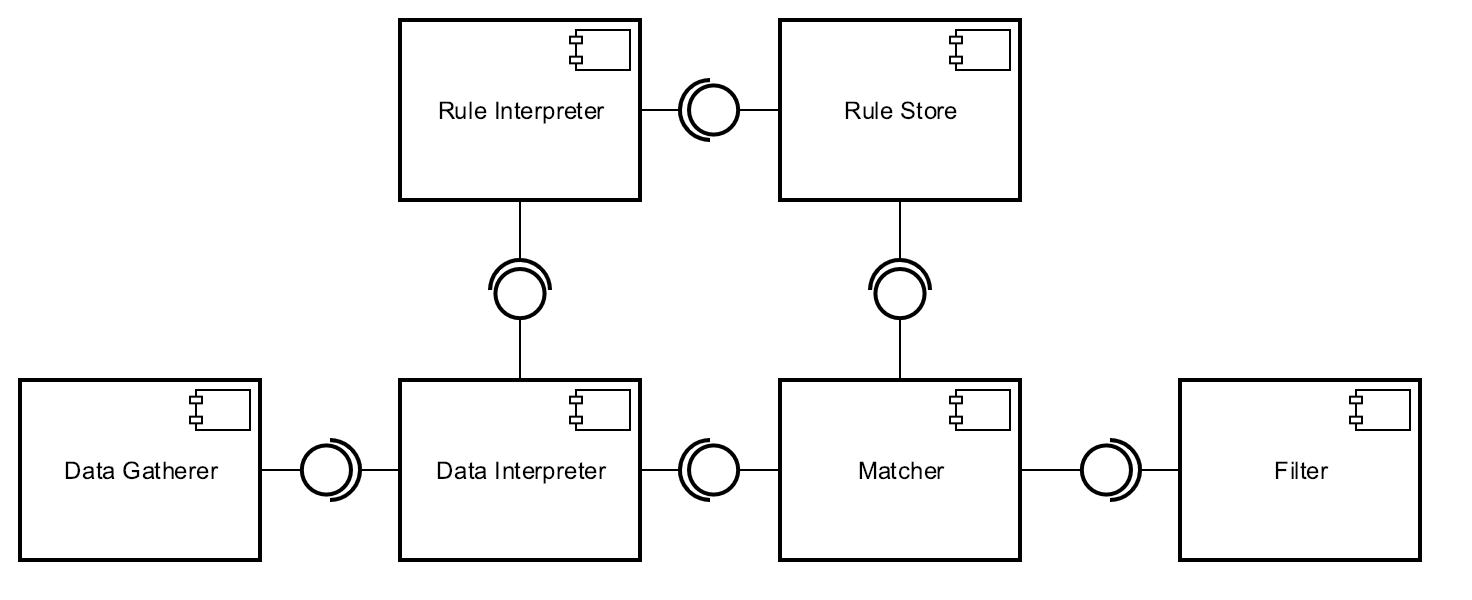
\includegraphics[width=\textwidth]{resources/behavior_based_architecture.png}
	\caption{Diagram Arsitektur \textit{Logical} Sistem}
	\label{fig:architecture_diagram}
\end{figure}

Arsitektur \textit{logical} sistem pada tugas akhir ini dapat dilihat pada diagram \ref{fig:architecture_diagram}. Perbedaan dari gagasan (\cite{6620049}) adalah pada \textit{data interpreter}, \textit{rule interpreter}, \textit{rule store} dan \textit{filter}. Secara garis besar berikut adalah tanggung jawab masing-masing komponen. \textit{Rule store} merupakan komponen yang bertanggung jawab untuk menyimpan dan menyediakan rule yang dibutuhkan oleh matcher. Kemudian \textit{rule interpreter} merupakan komponen yang bertanggung jawab untuk merepresentasikan rule untuk digunakan \textit{data interpreter}. Kemudian \textit{data interpreter} sebagai komponen yang bertanggung jawab untuk mengubah data yang diterima dari \textit{data gatherer} menjadi representasi masukan dari \textit{matcher}. Komponen \textit{filter} kemudian menjadi komponen penentu penyaring perilaku yang tidak diperbolehkan.

Komponen \textit{data interpreter} pada tugas akhir ini berfungsi menerima data dari \textit{data gatherer} kemudian mengubahnya dalam bentuk \textit{boolean} berdasarkan informasi yang diterima dari \textit{rule interpreter}. Pada dasarnya \textit{data interpreter} ini merupakan \textit{signature matcher} untuk \textit{input}. Nantinya, kumpulan \textit{signature} ini digunakan komponen \textit{matcher} untuk menentukan apakah ini merupakan perilaku berbahaya atau tidak.

Dengan menggunakan keluaran dari \textit{data interpreter}, komponen \textit{matcher} menentukan keputusan. Komponen ini melakukan pencocokan urutan signature terjadi dengan \textit{rule} yang dimiliki. Urutan signature terjadi tersebut berupa state machine yang disimpan oleh komponen \textit{rule store}.

Komponen-komponen ini kemudian harus dapat memenuhi kebutuhan yang telah disebutkan sebelumnya. Komponen \textit{data interpreter} merupakan bagian yang akan memiliki fungsionalitas untuk memenuhi kebutuhan SR3 dan SR4. Sedangkan komponen \textit{matcher} menjadi bagian penting yang memiliki fungsionalitas untuk menyimpan dan merespons input yakni SR2. Komponen \textit{filter} memiliki peran untuk memenuhi kebutuhan SR1. Kemudian komponen \textit{rule store} memiliki fungsionalitas untuk memenuhi kebutuhan SR5. Traceability tersebut dapat dilihat pada tabel \ref{table:system_traceability_design}.

\begin{table}[H]
	\caption{Traceability desain sistem}
	\label{table:system_traceability_design}
	\begin{tabularx}{\textwidth}{|l|X|X|}
		\hline
		\textbf{No} & \textbf{Kebutuhan} & \textbf{Komponen} \\ \hline
		SR1 & Penangkalan paket & komponen \textit{filter} \\ \hline 
		SR2 & State machine &  komponen \textit{matcher} \\ \hline
		SR3 & Deteksi protokol level aplikasi & komponen \textit{data interpreter} \\ \hline
		SR4 & Deteksi signature yang paham terhadap struktur data& komponen \textit{data interpreter} \\ \hline
		SR5 & Menambahkan rule & komponen \textit{rule store} \\ \hline
	\end{tabularx}
\end{table}

\section{Perancangan Rule dengan Iptables}

Pada bagian ini dibahas bagaimana rancangan rule iptables untuk menangkal WannaCry. Rule dibuat dari hasil analisis yang telah dilakukan pada subbab analisis perilaku malware WannaCry. Rancangan dilakukan dengan membuat state transition diagram untuk dijalankan pada state machine yang telah dibahas pada subbab sebelumnya.

Seperti telah dibahas pada bagian analisis, rule akan diimplementasi dengan membuat sebuah state transition sebuah koneksi \verb|SMB|. State transition diagram \ref{fig:state_transition_diagram} menggunakan perintah SMB sebagai alfabet masukan dan memiliki 3 state.

Seluruh koneksi pada awalnya berada pada state 0, dan akan terus pada state 0 hingga ditemukan signature bahwa koneksi merupakan koneksi SMB. Jika ditemukan signature, maka koneksi akan berubah menjadi state 1. Pada state 1 setiap paket akan dilakukan pengecekan terhadap command yang dilakukan. Jika ditemukan command \verb|COM_NT_TRANSACT| maka koneksi akan menjadi state 2. Kemudian state 2 ini merupakan state yang menentukan apakah ditemukan paket malicious yakni dengan mengirimkan \verb|COM_TRANSACTION2_SECONDARY| setelah \verb|COM_NT_TRANSACT|. Jika ditemukan maka koneksi akan ditandai untuk dilakukan \verb|DROP|.

\begin{figure}[H]
	\centering
	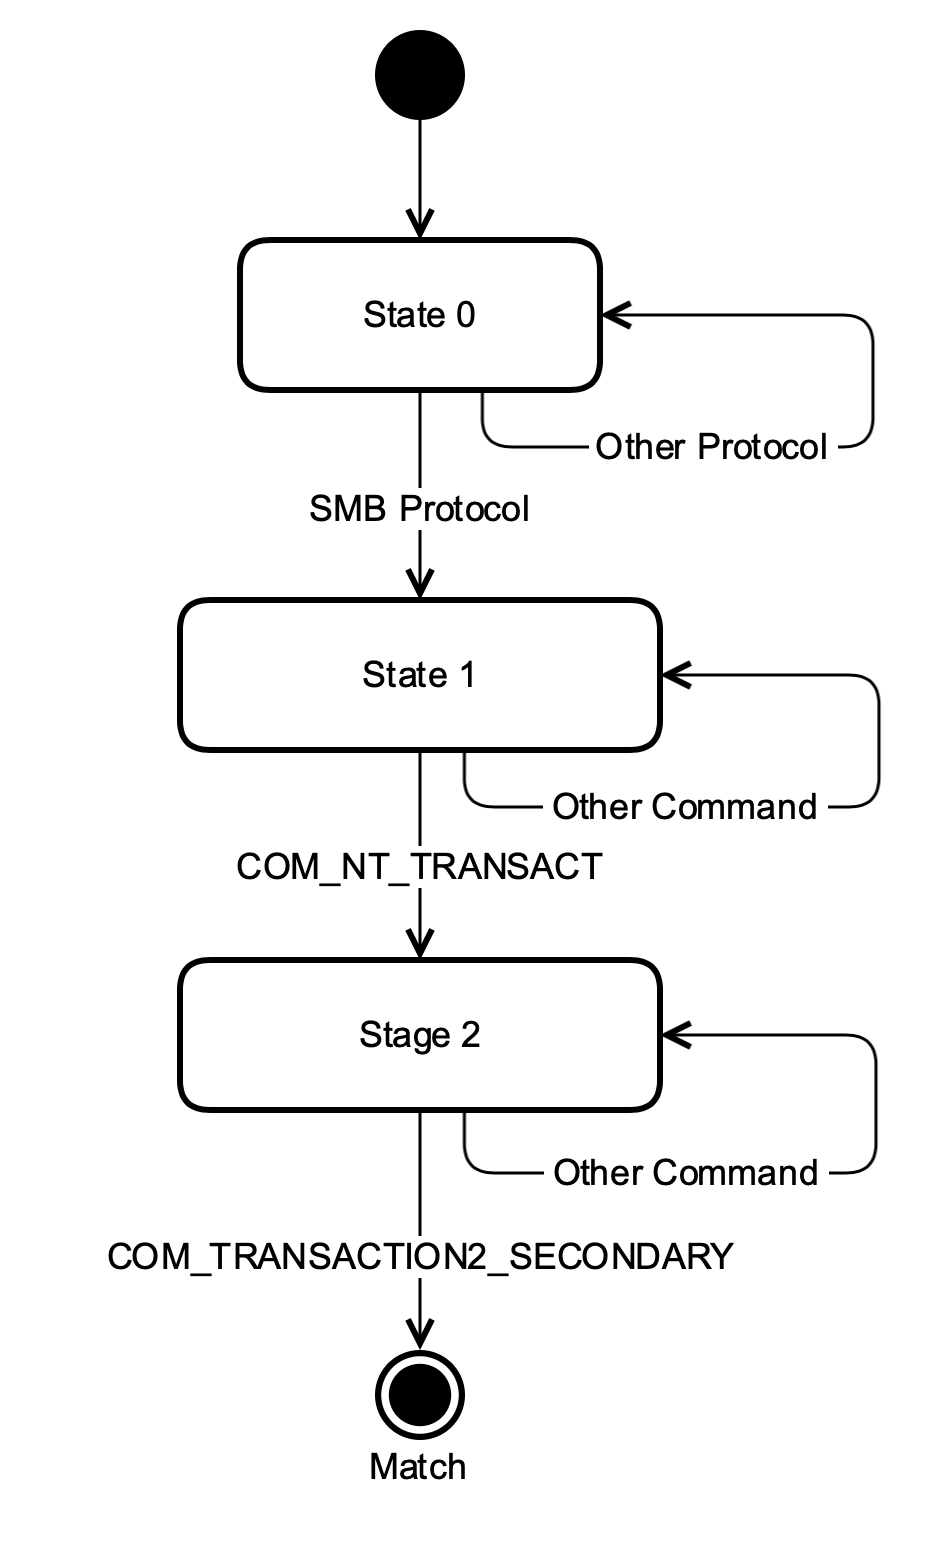
\includegraphics[width=200px]{resources/ngfilter_state_diagram.png}
	\caption{\textit{State Transition Diagram}}
	\label{fig:state_transition_diagram}
\end{figure}
